
\def\slidemode{%
  \documentclass[fleqn,aspectratio=169]{beamer}
}
\def\handoutmode{%
  \documentclass[handout,fleqn,aspectratio=169]{beamer}

}

\def\slidemode{
  \documentclass[fleqn,aspectratio=169]{beamer}
\usepackage{pgfpages}
}
\def\handoutmode{
  \documentclass[handout,fleqn,aspectratio=169]{beamer}
\usepackage{pgfpages}
\pgfpagesuselayout{resize to}[a4paper,landscape,border shrink=5mm]
}


%\def\pdfmode{handoutmode}
\def\pdfmode{slidemode}

\csname\pdfmode\endcsname

\usepackage{pgfpages}
\pgfpagesuselayout{resize to}[a4paper,landscape,border shrink=5mm]

\mode<presentation>
{
  \usetheme{default}
  \usecolortheme{default}
  \usefonttheme{default}
  \setbeamertemplate{navigation symbols}{}
  \setbeamertemplate{caption}[numbered]
  \setbeamertemplate{footline}[frame number]  % or "page number"
  \setbeamercolor{frametitle}{fg=white}
  \setbeamercolor{footline}{fg=black}
} 

\usepackage[english]{babel}
%\usepackage[utf8x]{inputenc}
\usepackage{tikz}
\usepackage{courier}
\usepackage{array}
\usepackage{bold-extra}
% \usepackage{minted}
% \usepackage[thicklines]{cancel}
%\usepackage{fancyvrb}
\usepackage{kotex}
\usepackage{paralist}
\usepackage{collectbox}

\setbeamercolor{block body alerted}{bg=alerted text.fg!10}
\setbeamercolor{block title alerted}{bg=alerted text.fg!20}
\setbeamercolor{block body}{bg=structure!10}
\setbeamercolor{block title}{bg=structure!20}
\setbeamercolor{block body example}{bg=green!10}
\setbeamercolor{block title example}{bg=green!20}
\setbeamertemplate{blocks}[rounded][shadow]

\xdefinecolor{dianablue}{rgb}{0.18,0.24,0.31}
\xdefinecolor{darkblue}{rgb}{0.1,0.1,0.7}
\xdefinecolor{darkgreen}{rgb}{0,0.5,0}
\xdefinecolor{darkgrey}{rgb}{0.35,0.35,0.35}
\xdefinecolor{darkorange}{rgb}{0.8,0.5,0}
\xdefinecolor{darkred}{rgb}{0.7,0,0}
\definecolor{darkgreen}{rgb}{0,0.6,0}
\definecolor{mauve}{rgb}{0.58,0,0.82}


\title[]{Lecture 3: Random Variable, Part I}
\author{Yi, Yung (이융)}
\institute{EE210: Probability and Introductory Random Processes\\ KAIST EE}
\date{\today}

\usetikzlibrary{shapes.callouts}

%%%%%%%%%%%% real, integer notation
\newcommand{\real}{{\mathbb R}}
\newcommand{\integer}{{\mathbb Z}}

%%% set, vector, matrix
\newcommand{\set}[1]{\ensuremath{\mathcal #1}}
\renewcommand{\vec}[1]{\bm{#1}}
\newcommand{\mat}[1]{\bm{#1}}


%%% big parenthesis
\def\Bl{\Bigl}
\def\Br{\Bigr}
\def\lf{\left}
\def\ri{\right}


%%% floor notations
\newcommand{\lfl}{{\lfloor}}
\newcommand{\rfl}{{\rfloor}}
\newcommand{\floor}[1]{{\lfloor #1 \rfloor}}

%%% gradient
\newcommand{\grad}[1]{\nabla #1}

%%% definition
\newcommand{\eqdef}{\ensuremath{\triangleq}}
%%% imply
\newcommand{\imp}{\Longrightarrow}



\newcommand{\separator}{
%  \begin{center}
    \par\noindent\rule{\columnwidth}{0.3mm}
%  \end{center}
}

\newcommand{\mynote}[1]{{\it \color{red} [#1]}}







%%% equation alignment
\newcommand{\aleq}[1]{\begin{align*}#1\end{align*}}

%%%%%%%%%%%%%%%% colored emphasized font, blanked words

\newcommand{\empr}[1]{{\color{red}\emph{#1}}}
\newcommand{\empb}[1]{{\color{blue}\emph{#1}}}

%normal colored text
\newcommand{\redf}[1]{{\color{red} #1}}
\newcommand{\yellowf}[1]{{\color{yellow} #1}}
\newcommand{\bluef}[1]{{\color{blue} #1}}
\newcommand{\grayf}[1]{{\color{gray} #1}}
\newcommand{\magenf}[1]{{\color{magenta} #1}}
\newcommand{\greenf}[1]{{\color{green} #1}}
\newcommand{\cyanf}[1]{{\color{cyan} #1}}
\newcommand{\orangef}[1]{{\color{orange} #1}}


\newcommand{\blk}[1]{\underline{\mbox{\hspace{#1}}}}


\newcommand{\redblk}[1]{\framebox{\color{red} #1}}
\newcommand{\redblank}[2]{\framebox{\onslide<#1->{\color{red} #2}}}
\newcommand{\blueblk}[1]{\framebox{\color{blue} #1}}
\newcommand{\blueblank}[2]{\framebox{\onslide<#1->{\color{blue} #2}}}



\makeatletter
\newcommand{\mybox}{%
    \collectbox{%
        \setlength{\fboxsep}{1pt}%
        \fbox{\BOXCONTENT}%
    }%
}
\makeatother

\makeatletter
\newcommand{\lecturemark}{%
    \collectbox{%
        \setlength{\fboxsep}{1pt}%
        \fcolorbox{red}{yellow}{\BOXCONTENT}%
    }%
}
\makeatother

\usepackage{tcolorbox}
\newcommand{\mycolorbox}[1]{
\begin{tcolorbox}[colback=red!5!white,colframe=red!75!black]
#1
\end{tcolorbox}
}

%%%% figure inclusion
\newcommand{\mypic}[2]{
\begin{center}
\includegraphics[width=#1\textwidth]{#2}
\end{center}
}

\newcommand{\myinlinepic}[2]{
\makebox[0cm][r]{\raisebox{-4ex}{\includegraphics[height=#1]{#2}}}
}


%%%% itemized and enumerated list
\newcommand{\bci}{\begin{compactitem}}
\newcommand{\eci}{\end{compactitem}}
\newcommand{\bce}{\begin{compactenum}}
\newcommand{\ece}{\end{compactenum}}


%%%% making 0.5/0.5 two columns
%%%% how to use: first number: length of separation bar
% \mytwocols{0.6}
% {
% contents in the left column
% }
% {
% contents in the right column
% }
%%%%
\newcommand{\mytwocols}[3]{
\begin{columns}[T] \column{.499\textwidth} #2 \column{.001\textwidth} \rule{.3mm}{{#1}\textheight} \column{.499\textwidth} #3 \end{columns}}

\newcommand{\mythreecols}[4]{
\begin{columns}[T] \column{.31\textwidth} #2 \column{.001\textwidth} \rule{.3mm}{{#1}\textheight} \column{.31\textwidth} #3 \column{.001\textwidth} \rule{.3mm}{{#1}\textheight} \column{.31\textwidth} #4  \end{columns}}

\newcommand{\mysmalltwocols}[3]{
\begin{columns}[T] \column{.4\textwidth} #2 \column{.001\textwidth} \rule{.3mm}{{#1}\textheight} \column{.4\textwidth} #3 \end{columns}}

%%%% making two columns with customized ratios
%%%% how to use:
%first parameter: length of separation bar
%second parameter: ratio of left column
%third parameter: ratio of right column
% \mytwocols{0.6}{0.7}{0.29}
% {
% contents in the left column
% }
% {
% contents in the right column
% }
%%%%
\newcommand{\myvartwocols}[5]{
\begin{columns}[T] \column{#2\textwidth} {#4} \column{.01\textwidth} \rule{.3mm}{{#1}\textheight} \column{#3\textwidth} {#5} \end{columns}}

%%% making my block in beamer
%%% first parameter: title of block
%%% second parameter: contents of block
\newcommand{\myblock}[2]{
\begin{block}{#1} {#2}  \end{block}}

%%% independence notation
\newcommand{\indep}{\perp \!\!\! \perp}

%%%% probability with different shapes (parenthesis or bracket) and different sizes
%%% `i' enables us to insert the subscript to the probability
\newcommand{\bprob}[1]{\mathbb{P}\Bl[ #1 \Br]}
\newcommand{\prob}[1]{\mathbb{P}[ #1 ]}
\newcommand{\cbprob}[1]{\mathbb{P}\Bl( #1 \Br)}
\newcommand{\cprob}[1]{\mathbb{P}( #1 )}
\newcommand{\probi}[2]{\mathbb{P}_{#1}[ #2 ]}
\newcommand{\bprobi}[2]{\mathbb{P}_{#1}\Bl[ #2 \Br]}
\newcommand{\cprobi}[2]{\mathbb{P}_{#1}( #2 )}
\newcommand{\cbprobi}[2]{\mathbb{P}_{#1}\Bl( #2 \Br)}

%%%% expectation with different shapes (parenthesis or bracket) and different sizes
%%% `i' enables us to insert the subscript to the expectation
\newcommand{\expect}[1]{\mathbb{E}[ #1 ]}
\newcommand{\cexpect}[1]{\mathbb{E}( #1 )}
\newcommand{\bexpect}[1]{\mathbb{E}\Bl[ #1 \Br]}
\newcommand{\cbexpect}[1]{\mathbb{E}\Bl( #1 \Br)}
\newcommand{\bbexpect}[1]{\mathbb{E}\lf[ #1 \ri]}
\newcommand{\expecti}[2]{\mathbb{E}_{#1}[ #2 ]}
\newcommand{\bexpecti}[2]{\mathbb{E}_{#1}\Bl[ #2 \Br]}
\newcommand{\bbexpecti}[2]{\mathbb{E}_{#1}\lf[ #2 \ri]}

%%%% variance
\newcommand{\var}[1]{\text{var}[ #1 ]}
\newcommand{\bvar}[1]{\text{var}\Bl[ #1 \Br]}
\newcommand{\cvar}[1]{\text{var}( #1 )}
\newcommand{\cbvar}[1]{\text{var}\Bl( #1 \Br)}

%%%% covariance
\newcommand{\cov}[1]{\text{cov}( #1 )}
\newcommand{\bcov}[1]{\text{cov}\Bl( #1 \Br)}

%%% Popular pmf, pdf notation to avoid long typing
\newcommand{\px}{\ensuremath{p_X(x)}}
\newcommand{\py}{\ensuremath{p_Y(y)}}
\newcommand{\pz}{\ensuremath{p_Z(z)}}
\newcommand{\pxA}{\ensuremath{p_{X|A}(x)}}
\newcommand{\pyA}{\ensuremath{p_{Y|A}(y)}}
\newcommand{\pzA}{\ensuremath{p_{Z|A}(z)}}
\newcommand{\pxy}{\ensuremath{p_{X,Y}(x,y)}}
\newcommand{\pxcy}{\ensuremath{p_{X|Y}(x|y)}}
\newcommand{\pycx}{\ensuremath{p_{Y|X}(y|x)}}

\newcommand{\fx}{\ensuremath{f_X(x)}}
\newcommand{\Fx}{\ensuremath{F_X(x)}}
\newcommand{\fy}{\ensuremath{f_Y(y)}}
\newcommand{\Fy}{\ensuremath{F_Y(y)}}
\newcommand{\fz}{\ensuremath{f_Z(z)}}
\newcommand{\Fz}{\ensuremath{F_Z(z)}}
\newcommand{\fxA}{\ensuremath{f_{X|A}(x)}}
\newcommand{\fyA}{\ensuremath{f_{Y|A}(y)}}
\newcommand{\fzA}{\ensuremath{f_{Z|A}(z)}}
\newcommand{\fxy}{\ensuremath{f_{X,Y}(x,y)}}
\newcommand{\Fxy}{\ensuremath{F_{X,Y}(x,y)}}
\newcommand{\fxcy}{\ensuremath{f_{X|Y}(x|y)}}
\newcommand{\fycx}{\ensuremath{f_{Y|X}(y|x)}}

\newcommand{\fth}{\ensuremath{f_\Theta(\theta)}}
\newcommand{\fxcth}{\ensuremath{f_{X|\Theta}(x|\theta)}}
\newcommand{\fthcx}{\ensuremath{f_{\Theta|X}(\theta|x)}}

\newcommand{\pkcth}{\ensuremath{p_{X|\Theta}(k|\theta)}}
\newcommand{\fthck}{\ensuremath{f_{\Theta|X}(\theta|k)}}


%%%% indicator
\newcommand{\indi}[1]{\mathbf{1}_{ #1 }}

%%%% exponential rv.
\newcommand{\elambdax}{\ensuremath{e^{-\lambda x}}}

%%%% normal  rv.
\newcommand{\stdnormal}{\ensuremath{\frac{1}{\sqrt{2\pi}} e^{-x^2/2}}}
\newcommand{\gennormal}{\ensuremath{\frac{1}{\sigma\sqrt{2\pi}} e^{-(x-\mu)^2/2}}}

%%%%%% estimator, estimate
\newcommand{\hth}{\ensuremath{\hat{\theta}}}
\newcommand{\hTH}{\ensuremath{\hat{\Theta}}}
\newcommand{\MAP}{\ensuremath{\text{MAP}}}
\newcommand{\LMS}{\ensuremath{\text{LMS}}}
\newcommand{\LLMS}{\ensuremath{\text{L}}}
\newcommand{\ML}{\ensuremath{\text{ML}}}

%%%% colored text
\newcommand{\red}[1]{\color{red}#1}
\newcommand{\cyan}[1]{\color{cyan}#1}
\newcommand{\magenta}[1]{\color{magenta}#1}
\newcommand{\blue}[1]{\color{blue}#1}
\newcommand{\green}[1]{\color{green}#1}
\newcommand{\white}[1]{\color{white}#1}

\newcommand{\defi}{{\color{red} Definition.} }
\newcommand{\proff}{{\color{red} Proof.} }
\newcommand{\exam}{{\color{red} Example.} }
\newcommand{\question}{{\color{red} Question.} }
\newcommand{\thm}{{\color{red} Theorem.} }
\newcommand{\background}{{\color{red} Background.} }
\newcommand{\msg}{{\color{red} Message.} }

\newcommand{\bern}[1]{\ensuremath{\text{Bern}(#1)} }
\newcommand{\bp}[1]{\ensuremath{\text{BP}(#1)} }
\newcommand{\poisson}[1]{\ensuremath{\text{Poisson}(#1)} }
\newcommand{\pp}[1]{\ensuremath{\text{PP}(#1)} }


%%%%%%%%%%%%%%%%%%%%%%% old macros that you can ignore %%%%%%%%%%%%%%%%%%%%%%%%

% \def\un{\underline}
% \def\ov{\overline}


% \newcommand{\beq}{\begin{eqnarray*}}
% \newcommand{\eeq}{\end{eqnarray*}}
% \newcommand{\beqn}{\begin{eqnarray}}
% \newcommand{\eeqn}{\end{eqnarray}}
% \newcommand{\bemn}{\begin{multiline}}
% \newcommand{\eemn}{\end{multiline}}
% \newcommand{\beal}{\begin{align}}
% \newcommand{\eeal}{\end{align}}
% \newcommand{\beas}{\begin{align*}}
% \newcommand{\eeas}{\end{align*}}



% \newcommand{\bd}{\begin{displaymath}}
% \newcommand{\ed}{\end{displaymath}}
% \newcommand{\bee}{\begin{equation}}
% \newcommand{\eee}{\end{equation}}


% \newcommand{\vs}{\vspace{0.2in}}
% \newcommand{\hs}{\hspace{0.5in}}
% \newcommand{\el}{\end{flushleft}}
% \newcommand{\bl}{\begin{flushleft}}
% \newcommand{\bc}{\begin{center}}
% \newcommand{\ec}{\end{center}}
% \newcommand{\remove}[1]{}

% \newtheorem{theorem}{Theorem}
% \newtheorem{corollary}{Corollary}
% \newtheorem{prop}{Proposition}
% \newtheorem{lemma}{Lemma}
% \newtheorem{defi}{Definition}
% \newtheorem{assum}{Assumption}
% \newtheorem{example}{Example}
% \newtheorem{property}{Property}
% \newtheorem{remark}{Remark}

% \newcommand{\separator}{
%   \begin{center}
%     \rule{\columnwidth}{0.3mm}
%   \end{center}
% }

% \newenvironment{separation}
% { \vspace{-0.3cm}
%   \separator
%   \vspace{-0.25cm}
% }
% {
%   \vspace{-0.5cm}
%   \separator
%   \vspace{-0.15cm}
% }

% \def\A{\mathcal A}
% \def\oA{\overline{\mathcal A}}
% \def\S{\mathcal S}
% \def\D{\mathcal D}
% \def\eff{{\rm Eff}}
% \def\bD{\bm{D}}
% \def\cU{{\cal U}}
% \def\bbs{{\mathbb{s}}}
% \def\bbS{{\mathbb{S} }}
% \def\cM{{\cal M}}
% \def\bV{{\bm{V}}}
% \def\cH{{\cal H}}
% \def\ch{{\cal h}}
% \def\cR{{\cal R}}
% \def\cV{{\cal V}}
% \def\cA{{\cal A}}
% \def\cX{{\cal X}}
% \def\cN{{\cal N}}
% \def\cJ{{\cal J}}
% \def\cK{{\cal K}}
% \def\cL{{\cal L}}
% \def\cI{{\cal I}}
% \def\cY{{\cal Y}}
% \def\cZ{{\cal Z}}
% \def\cC{{\cal C}}
% \def\cR{{\cal R}}
% \def\id{{\rm Id}}
% \def\st{{\rm st}}
% \def\cF{{\cal F}}
% \def\bz{{\bm z}}
% \def\cG{{\cal G}}
% \def\N{\mathbb{N}}
% \def\bbh{\mathbb{h}}
% \def\bbH{\mathbb{H}}
% \def\bbi{\mathbb{i}}
% \def\bbI{\mathbb{I}}
% \def\R{\mathbb{R}}
% \def\bbR{\mathbb{R}}
% \def\bbr{\mathbb{r}}
% \def\cB{{\cal B}}
% \def\cP{{\cal P}}
% \def\cS{{\cal S}}
% \def\bW{{\bm W}}
% \def\bc{{\bm c}}

% %\def\and{\quad\mbox{and}\quad}
% \def\ind{{\bf 1}}


% \def\bmg{{\bm{\gamma}}}
% \def\bmr{{\bm{\rho}}}
% \def\bmq{{\bm{q}}}
% \def\bmt{{\bm{\tau}}}
% \def\bmn{{\bm{n}}}
% \def\bmcapn{{\bm{N}}}
% \def\bmrho{{\bm{\rho}}}

% \def\igam{\underline{\gamma}(\lambda)}
% \def\sgam{\overline{\gamma}(\lambda)}
% \def\ovt{\overline{\theta}}
% \def\ovT{\overline{\Theta}}
% \def\PP{{\mathrm P}}
% \def\EE{{\mathrm E}}
% \def\iskip{{\vskip -0.4cm}}
% \def\siskip{{\vskip -0.2cm}}

% \def\bp{\noindent{\it Proof.}\ }
% \def\ep{\hfill $\Box$}



\begin{document}

%itemshape
\setbeamertemplate{itemize item}{\scriptsize\raise1.25pt\hbox{\donotcoloroutermaths$\bullet$}}
\setbeamertemplate{itemize subitem}{\tiny\raise1.5pt\hbox{\donotcoloroutermaths$\circ$}}
\setbeamertemplate{itemize subsubitem}{\tiny\raise1.5pt\hbox{\donotcoloroutermaths$\blacktriangleright$}}
%default value for spacing
\plitemsep 0.1in
\pltopsep 0.03in
\setlength{\parskip}{0.15in}
%\setlength{\parindent}{-0.5in}
\setlength{\abovedisplayskip}{0.07in}
\setlength{\mathindent}{0cm}
\setbeamertemplate{frametitle continuation}{[\insertcontinuationcount]}

\setlength{\leftmargini}{0.5cm}
\setlength{\leftmarginii}{0.5cm}

\setlength{\fboxrule}{0.05pt}
\setlength{\fboxsep}{5pt}

\logo{\pgfputat{\pgfxy(0.11, 7.4)}{\pgfbox[right,base]{\tikz{\filldraw[fill=dianablue, draw=none] (0 cm, 0 cm) rectangle (50 cm, 1 cm);}\mbox{\hspace{-8 cm}
\includegraphics[height=0.7 cm]{../kaist_ee.png}
}}}}

\begin{frame}
  \titlepage
\end{frame}

\logo{\pgfputat{\pgfxy(0.11, 7.4)}{\pgfbox[right,base]{\tikz{\filldraw[fill=dianablue, draw=none] (0 cm, 0 cm) rectangle (50 cm, 1 cm);}\mbox{\hspace{-8 cm}
\includegraphics[height=0.7 cm]{../kaist_ee.png}
}}}}

% Uncomment these lines for an automatically generated outline.
\begin{frame}{Outline}

\bci
\item Random Variable: Discrete

\item PMF (Probability Mass Function)

\item Representative Discrete Random Variables

\item Expectation and Variance

\item Functions of Random Variables

\item Conditioning and Independence for Random Variables
\eci
\end{frame}

% START START START START START START START START START START START START START

%%%%%%%%%%%%%%%%%%%%%%%%%%%%%%%%%%%%%%%%%%%%%%%%%%%%%%
\begin{frame}{Random Variable: Idea}


\myvartwocols{0.7}{0.4}{0.57}
{
\plitemsep 0.1in

\bci 
\item In reality, many outcomes are \redblank{2}{numerical}, e.g., stock price.

\item Even if not, very convenient if we map numerical values to random outcomes, e.g., `0' for male and `1' for female.

\eci 
}
{
\centering
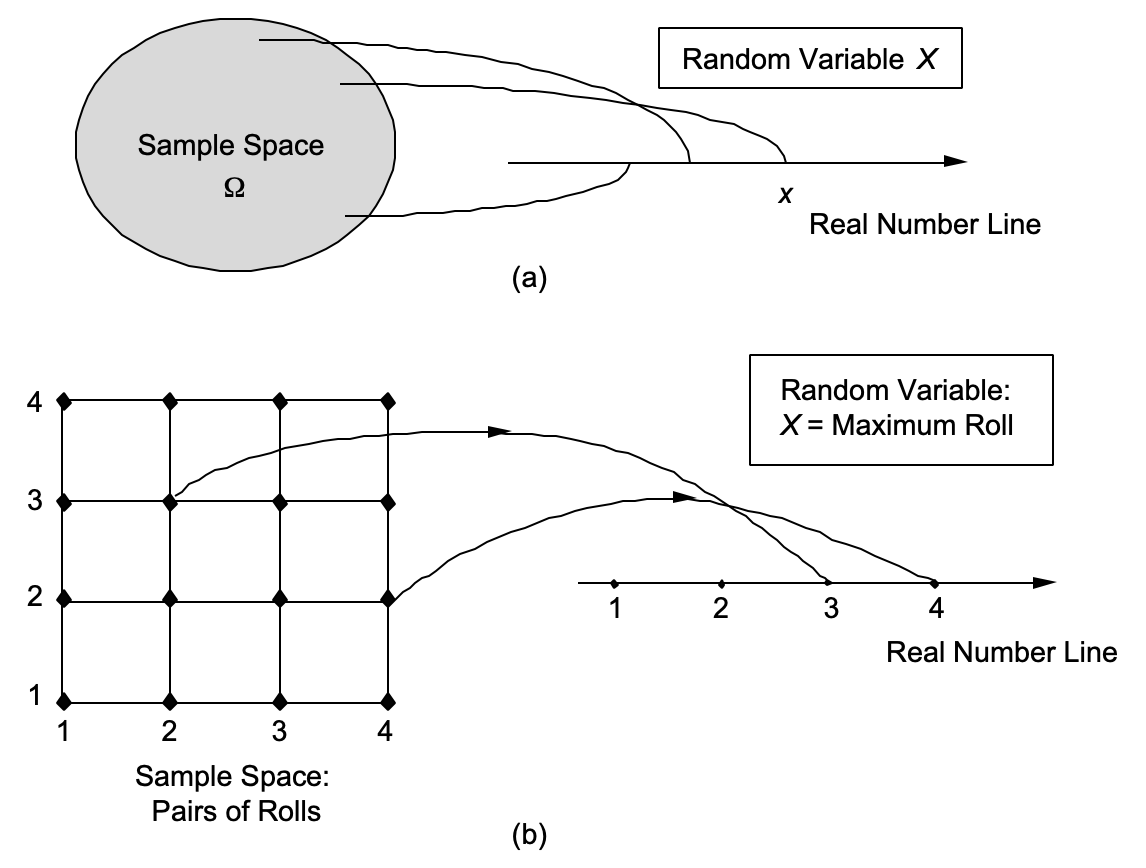
\includegraphics[width=0.9\textwidth]{L3_RV_ex.png}
}

\end{frame}

%%%%%%%%%%%%%%%%%%%%%%%%%%%%%%%%%%%%%%%%%%%%%%%%%%%%%%
\begin{frame}{Random Variable: More Formally}

\plitemsep 0.1in

\bci [$\circ$]
\item<2-> Mathematically, a random variable $X$ is a \redblank{3}{function} which maps from $\Omega$ to $\real.$

\item<4-> \bluef{Notation.} Random variable $X$, numerical value $x.$

\item<5-> Different random variables $X$, $Y,$, etc can be defined on the same sample space. 

\item<6-> For a fixed value $x,$ we can associate an \redblank{7}{event} that a random variable $X$ has the value $x,$ i.e., 
\redblank{8}{$\{ \omega \in \Omega \mid X(w) = x \}$}

\item<8-> Assume that values $x$ are discrete\footnote{Finite or countably infinite.} such as $1, 2, 3, \ldots.$

For notational convenience,  
$$
p_X(x) \ \eqdef \ \cprob{X = x} \ \eqdef \ \cbprob{\{ \omega \in \Omega \mid X(w) = x \}} 
$$

\item<9-> For a discrete random variable $X$, we call $p_X(x)$ \redblank{10}{probability mass function} (PMF).

\eci 

\end{frame}

%%%%%%%%%%%%%%%%%%%%%%%%%%%%%%%%%%%%%%%%%%%%%%%%%%%%%%
\begin{frame}{Roadmap}

\plitemsep 0.1in

\bci 
\item Famous discrete random variables used in the community

- Bernoulli, Uniform, Binomial, Geometric, Poisson, etc. 

\item Summarizing a random variable: Expectation and Variance

\item Functions of a single random variable, Functions of multiple random variables 

\item Conditioning for random variables, Independence for random variables 

\item Continuous random variables

- Normal, Uniform, Exponential, etc. 

\item Bayes' rule for random variables
\eci 

\end{frame}

%%%%%%%%%%%%%%%%%%%%%%%%%%%%%%%%%%%%%%%%%%%%%%%%%%%%%%
\begin{frame}{Roadmap}

\plitemsep 0.1in

\bci [$\circ$]
\item \redf{Famous discrete random variables used in the community

- Bernoulli, Uniform, Binomial, Geometric, Poisson, etc. }

\item Summarizing a random variable: Expectation and Variance

\item Functions of a single random variable, Functions of multiple random variables 

\item Conditioning for random variables, Independence for random variables 

\item Continuous random variables

- Normal, Uniform, Exponential, etc. 

\item Bayes' rule for random variables
\eci 

\end{frame}

% %%%%%%%%%%%%%%%%%%%%%%%%%%%%%%%%%%%%%%%%%%%%%%%%%%%%%%
% \begin{frame}{}
% \vspace{2cm}
% \LARGE Examples of Famous Discrete Random Variables

% \end{frame}

%%%%%%%%%%%%%%%%%%%%%%%%%%%%%%%%%%%%%%%%%%%%%%%%%%%%%%
\begin{frame}{Bernoulli $X$ with parameter $p \in [0,1]$}

\plitemsep 0.1in

\bci
\item<1-> Only \redf{binary} values
\onslide<2->{
$$
X = \begin{cases}
0, & \text{w.p.\footnotemark} \quad 1-p, \cr
1, & \text{w.p.} \quad p
\end{cases}
$$
In other words, $p_X(0)=1-p$ and $p_X(1)=p$ from our PMF notation. }
\footnotetext{with probability}

\item<3-> Models a trial that results in binary results, e.g., success/failure, head/tail

\item<4-> Very useful for an \redblank{5}{indicator rv} of an event $A.$ 
\onslide<5->{
Define a rv $\indi{A}$ as:
$$
\indi{A} = 
\begin{cases}
1, & \text{if $A$ occurs}, \cr
0, & \text{otherwise}
\end{cases}
$$
}
\eci 

\end{frame}

%%%%%%%%%%%%%%%%%%%%%%%%%%%%%%%%%%%%%%%%%%%%%%%%%%%%%%
\begin{frame}{Uniform $X$ with parameter $a,b$}

\plitemsep 0.1in

\bci 
\item integers $a,b$, where $a \le b$

\item<2-> Choose a number of $\Omega = \{ a, a+1, \ldots, b \}$ uniformly at random. 

\item<3-> $p_X(i) = \frac{1}{b-a+1},$ $i \in \Omega.$

%\item $X(\omega) = \omega$

\centering
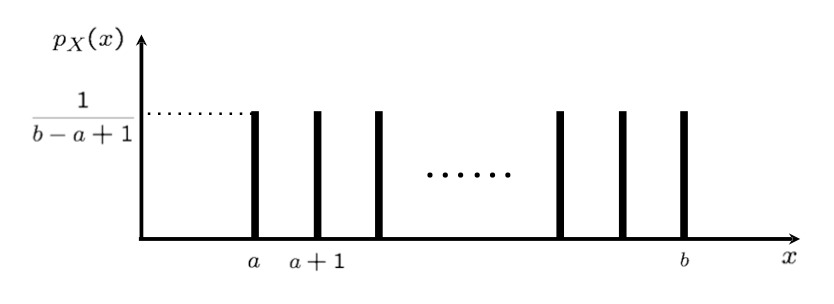
\includegraphics[width=0.7\textwidth]{L3_uniform_ex.png}

\item<4-> Models complete ignorance (I don't know anything about $X$)

\eci 

\end{frame}

%%%%%%%%%%%%%%%%%%%%%%%%%%%%%%%%%%%%%%%%%%%%%%%%%%%%%%
\begin{frame}{Binomial $X$ with parameter $n,p$}

\mytwocols{0.5}
{
\plitemsep 0.1in
\bci 
\item<2-> Models the number of successes in a given number of independent trials
\item<3-> $n$ independent trials, where one trial has the success probability $p.$

$$
p_X(k) = {n \choose k} p^k (1-p)^{n-k}
$$
\eci 
}
{
\centering
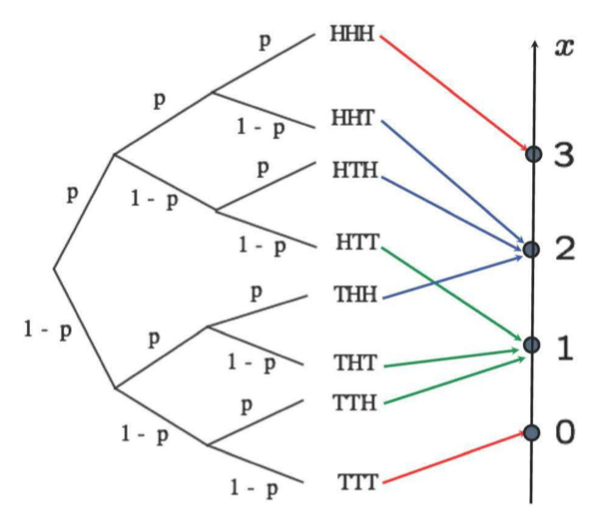
\includegraphics[width=0.8\textwidth]{L3_binomial_ex.png}
}
\end{frame}

%%%%%%%%%%%%%%%%%%%%%%%%%%%%%%%%%%%%%%%%%%%%%%%%%%%%%%
\begin{frame}{Poisson $X$ with parameter $\lambda$}

%\setdefaultleftmargin{0.1em}{}{}{}{}{}.

\plitemsep 0.05in
\bci 
\item<2-> $Binomial(n,p)$: Models the number of successes in a given number of independent trials with success probability $p.$

\item<3-> Very large $n$ and very small $p,$ such that $np =\lambda$
$$
p_X(k) = e^{-\lambda}\frac{\lambda^k}{k!}, \quad k=0,1, \ldots
$$

\item<4-> Is this a legitimate PMF?
\aleq{
\sum_{k=0}^\infty e^{-\lambda}\frac{\lambda^k}{k!} = e^{-\lambda} \left(1+ \lambda + \frac{\lambda^2}{2!} + \frac{\lambda^3}{3!} \ldots \right) = e^{-\lambda} e^\lambda = 1
}

\item<5-> Prove this:
$$
\lim_{n \rightarrow \infty} p_X(k) = {n \choose k} (1/n)^k (1-1/n)^{n-k} = e^{-\lambda}\frac{\lambda^k}{k!}
$$


\eci 

\end{frame}

%%%%%%%%%%%%%%%%%%%%%%%%%%%%%%%%%%%%%%%%%%%%%%%%%%%%%%
\begin{frame}{Geometric $X$ with parameter $p$}

\mytwocols{0.5}
{
\plitemsep 0.1in
\bci 
\item<1-> Experiment: infinitely many independent Bernoulli trials, where each trial has success probability $p$

\item<2-> Random variable: number of trials until the \redf{first success.} 

\item<3-> Models waiting times until something happens. 
$$
p_X(k) =  (1-p)^{k-1} p
$$
\eci 
}
{
\centering
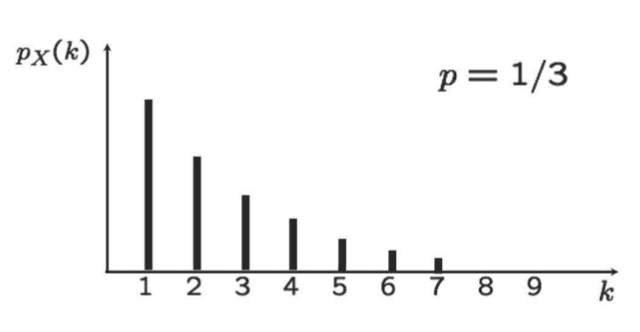
\includegraphics[width=0.8\textwidth]{L3_geo_ex.png}
}
\end{frame}

%%%%%%%%%%%%%%%%%%%%%%%%%%%%%%%%%%%%%%%%%%%%%%%%%%%%%%
\begin{frame}{Roadmap}

\plitemsep 0.1in

\bci
\item \bluef{Famous discrete random variables used in the community

- Bernoulli, Uniform, Binomial, Geometric, Poisson, etc. }

\item \redf{Summarizing a random variable: Expectation and Variance}

\item \redf{Functions of a single random variable}, Functions of multiple random variables 

\item Conditioning for random variables, Independence for random variables 

\item Continuous random variables

- Normal, Uniform, Exponential, etc. 

\item Bayes' rule for random variables
\eci 

\end{frame}


% %%%%%%%%%%%%%%%%%%%%%%%%%%%%%%%%%%%%%%%%%%%%%%%%%%%%%%
% \begin{frame}{}
% \vspace{2cm}
% \LARGE Summarizing Random Variables: Expectation and Variance

% \end{frame}

%%%%%%%%%%%%%%%%%%%%%%%%%%%%%%%%%%%%%%%%%%%%%%%%%%%%%%
\begin{frame}{Expectation/Mean}

\plitemsep 0.1in
\bci 
\item Average. 
\begin{block}{Definition}
$$
\expect{X} = \sum_{x} x p_X(x)
$$
\end{block}

\item $p_X(x)$: relative frequency of value $x$ (trials with $x$/total trials)

\item<2-> Example 1: Bernoulli r.v. with $p$
$$
\expect{X} = 1\times p + 0 \times (1-p) = p_X(1)
$$
\eci 

\end{frame}

%%%%%%%%%%%%%%%%%%%%%%%%%%%%%%%%%%%%%%%%%%%%%%%%%%%%%%
\begin{frame}{Properties of Expectation}

Not very surprising. Easy to prove using the definition.

\plitemsep 0.7in
\bci [$\circ$]

\item If $X \geq 0,$ $\expect{X} \geq 0.$

\item If $a \le X \le b,$ $a \le \expect{X} \le b.$

\item For a constant $c$, $\expect{c} = c.$
\eci 

\end{frame}

%%%%%%%%%%%%%%%%%%%%%%%%%%%%%%%%%%%%%%%%%%%%%%%%%%%%%%
\begin{frame}{Expectation of a function of a RV}

\plitemsep 0.05in
\bci 

\item<1-> For a rv $X,$ $Y =g (X)$ is also a r.v.

\item<2-> $\expect{Y} = \expect{g(X)} = \sum_{x} g(x) p_X(x)$ 

\item<3-> Compute $\expect{Y}$ for the following:

\mytwocols{0.4}{
\centering
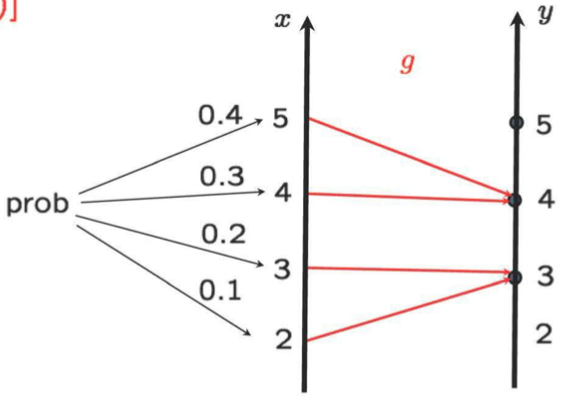
\includegraphics[width=0.7\textwidth]{L3_rvfunc_ex.png}
}
{
\onslide<4->{
\begin{multline*}
4\times (0.4+0.3) + 3 \times (0.1+0.2) \cr 
= 2.8 + 0.9 = 3.7
\end{multline*}
}
}

%\item Using the above,
\onslide<5->{
\myblock{Linearity of Expectation}
{$\expect{aX +b} = a\expect{X} + b$}
}
\eci 

\end{frame}

%%%%%%%%%%%%%%%%%%%%%%%%%%%%%%%%%%%%%%%%%%%%%%%%%%%%%%
\begin{frame}{Variance}

\plitemsep 0.1in
\bci 

\item<1-> Measures how much the \redblk{spread} of a PMF is. 

\item<2-> What about $\expect{X - \mu},$ where $\mu = \expect{X}$? Then, what about $\expect{(X - \mu)^2}$?


\myblock{Variance, Standard Deviation}
{
\onslide<3->{
\aleq{
    \var{X} &= \expect{(X-\mu)^2} \cr
    \sigma_X &= \sqrt{\var{X}}
}
}
}
% \item Useful formula
% $$
%     \var{X} = \expect{X^2} - (\expect{X})^2
% $$
\eci 

\end{frame}

%%%%%%%%%%%%%%%%%%%%%%%%%%%%%%%%%%%%%%%%%%%%%%%%%%%%%%
\begin{frame}{Variance: Useful Property}


\mytwocols{0.6}
{
\plitemsep 0.1in
\small

\bci 

\item  $\var{X} = \expect{X^2} - (\expect{X})^2$
\aleq{
\onslide<2->{
&\var{X} = \expect{X^2 - 2\mu X + \mu^2}\cr
&= \expect{X^2} -2\mu\expect{X} + \mu^2 = \expect{X^2} - \mu^2
}}
\item $Y= X+b$, $\var{Y} = \var{X}$
\aleq{
\onslide<3->{
\var{Y} = \expect{(X+b)^2} - (\expect{X+b})^2
}}

\item $Y = aX,$ $\var{Y} = a^2\var{X}$
\aleq{
\onslide<4->{
\var{Y} = \expect{a^2X^2} - (a\expect{X})^2
}
}


\eci 
}
{
Example: Variance of a Bernoulli rv ($p$)
\aleq{
\onslide<4->{
\expect{X} &= 1\times p + 0 \times (1-p) = p\cr
\expect{X^2}&= 1 \times p + 0 \times (1-p) = p \cr
\var{X} &= \expect{X^2} - \mu^2 = p - p^2\cr
&= p(1-p)
}
}

}
\end{frame}

%%%%%%%%%%%%%%%%%%%%%%%%%%%%%%%%%%%%%%%%%%%%%%%%%%%%%%
\begin{frame}{Roadmap}

\plitemsep 0.1in

\bci [$\circ$]
\item \bluef{Famous discrete random variables used in the community

- Bernoulli, Uniform, Binomial, Geometric, Poisson, etc. }

\item \bluef{Summarizing a random variable: Expectation and Variance}

\item \bluef{Functions of a single random variable}, \redf{Functions of multiple random variables} 

\item Conditioning for random variables, Independence for random variables 

\item Continuous random variables

- Normal, Uniform, Exponential, etc. 

\item Bayes' rule for random variables
\eci 

\end{frame}


%%%%%%%%%%%%%%%%%%%%%%%%%%%%%%%%%%%%%%%%%%%%%%%%%%%%%%
\begin{frame}{Joint PMF}

\mytwocols{0.75}
{
\plitemsep 0.1in
\bci 

\item<2-> \redblank{3}{Joint PMF.} For two random variables $X,Y,$ consider two events
$\{X = x \}$ and $\{Y = y \},$ and
\aleq{
\onslide<3->{\redf{\pxy} \ \eqdef} \ \cbprob{\{X = x \} \cap \{Y = y \}}
}
\item<4-> $\sum_x \sum_y \pxy = 1$

\item<5-> \redblank{6}{Marginal PMF.} 
\aleq{
    \px &= \sum_{y} \pxy, \cr
    \py &= \sum_{x} \pxy
}

\eci 
}
{
Example.

\medskip
\centering
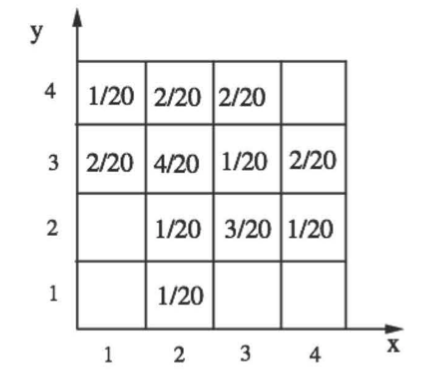
\includegraphics[width=0.5\textwidth]{L3_joint_ex.png}
\aleq{
p_{X,Y}(1,3)= 2/20
}
\aleq{
p_{X}(4) = 2/20 + 1/20 = 3/20
}
\aleq{
\cprob{X=Y}= 1/20 + 4/20 + 3/20 = 8/20
}
}
\end{frame}

%%%%%%%%%%%%%%%%%%%%%%%%%%%%%%%%%%%%%%%%%%%%%%%%%%%%%%
\begin{frame}{Functions of Multiple R.V.s}

\plitemsep 0.1in
\bci

\item<1-> Consider a rv $Z = g(X,Y).$ (Ex) $X+Y,$ $X^2 + Y^2.$  Then, PMF of $Z$ is:
$$
\onslide<2->{\pz = \cprob{g(X,Y) = z} = \sum_{(x,y): g(x,y) = z} \pxy}
$$

\item Similarly, 
$$
\expect{Z} = \expect{g(X,Y)} = \onslide<2->{\sum_{x} \sum_{y} g(x,y) \pxy}
$$


\eci 
\end{frame}


%%%%%%%%%%%%%%%%%%%%%%%%%%%%%%%%%%%%%%%%%%%%%%%%%%%%%%
\begin{frame}{Linearity of Expectation for multiple rvs }


\mytwocols{0.7}
{
\plitemsep 0.15in
\bci 

\item Remember: $\expect{aX + b} = a\expect{X} +b$

\item<2-> Similarly, 
$$\expect{X+Y} = \expect{X} + \expect{Y}$$ 
(easy to prove, using the definition.)

\bigskip

\bigskip

\item<3-> $\expect{X_1 \ldots + X_n} = \expect{X_1} + \ldots + \expect{X_n}$

\item<3-> $\expect{2X + 3Y - Z} = 2\expect{X} + 3 \expect{Y} - \expect{Z}$
\eci 
}
{
\plitemsep 0.15in
\bci 

\item<4-> \redf{Example.} Mean of a binomial rv $Y$ with $(n,p)$

\item<4-> $Y$: number of successes in $n$ Bernoulli trials with $p$

\item<5-> $Y = X_1 + \ldots X_n,$ where $X_i$ is a Bernoulli rv. 

\item<5-> $\expect{Y} = n \expect{X_i} = n \cprob{X_i = 1} = np$

\eci 

}
\end{frame}


%%%%%%%%%%%%%%%%%%%%%%%%%%%%%%%%%%%%%%%%%%%%%%%%%%%%%%
\begin{frame}{Roadmap}

\plitemsep 0.1in

\bci [$\circ$]
\item \bluef{Famous discrete random variables used in the community

- Bernoulli, Uniform, Binomial, Geometric, Poisson, etc. }

\item \bluef{Summarizing a random variable: Expectation and Variance}

\item \bluef{Functions of a single random variable}, \bluef{Functions of multiple random variables} 

\item \redf{Conditioning for random variables}, Independence for random variables 

\item Continuous random variables

- Normal, Uniform, Exponential, etc. 

\item Bayes' rule for random variables
\eci 

\end{frame}

%%%%%%%%%%%%%%%%%%%%%%%%%%%%%%%%%%%%%%%%%%%%%%%%%%%%%%
\begin{frame}{Conditional PMF: Conditioning on an event}

\onslide<1->{Remember two probability laws: $\cprob{\cdot}$ and $\cprob{\cdot | A},$ \bluef{for an event $A.$}}

\medskip

\mytwocols{0.7}
{
\plitemsep 0.2in
\bci 

\item<2-> $\px = \cprob{X=x}$

\item<3-> $\expect{X} = \sum_x x \px$

\item<4-> $\expect{g(X)} = \sum_x g(x) \px$

\item<5-> $\var{X} = \expect{X^2} - (\expect{X})^2$
\eci 
}
{
\plitemsep 0.2in
\bci 

\item<2-> $\redf{\pxA} \ \eqdef \ \cprob{X=x | A}$ 

\item<3-> $\redf{\expect{X | A}} \ \eqdef \ \sum_x x \pxA$

\item<4-> $\redf{\expect{g(X) | A}} \ \eqdef \ \sum_x g(x) \pxA$

\item<5-> $\redf{\var{X | A}} \ \eqdef \ \expect{X^2 |A } - (\expect{X|A})^2$

\medskip
\item<6-> \redf{Note.} $\pxA,$ $\expect{X | A}$, $\expect{g(X) | A},$ and $\var{X |A}$ are all just notations! 

\eci 
}

\end{frame}

%%%%%%%%%%%%%%%%%%%%%%%%%%%%%%%%%%%%%%%%%%%%%%%%%%%%%%
\begin{frame}{Example: Conditional PMF}

\hfill $A = \{X \geq 2 \}$

\medskip

\mytwocols{0.7}
{
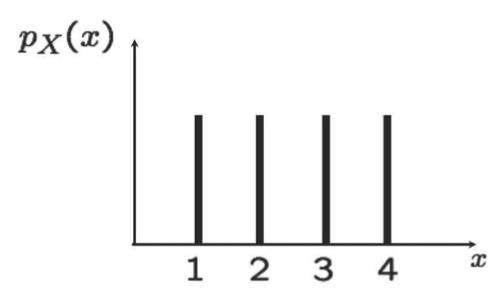
\includegraphics[width=0.55\textwidth]{L3_cond_pmf_ex1.png}

\medskip
\aleq{
\expect{X} = \onslide<2->{\frac{1}{4} \left( 1+2+3+4 \right) = 2.5}
}
\aleq{
\var{X} &= \onslide<3->{\expect{X^2} - (\expect{X})^2 \cr
&=\frac{1}{4}(1+2^2 +3^2+4^2) - 2.5^2}
}
}
{
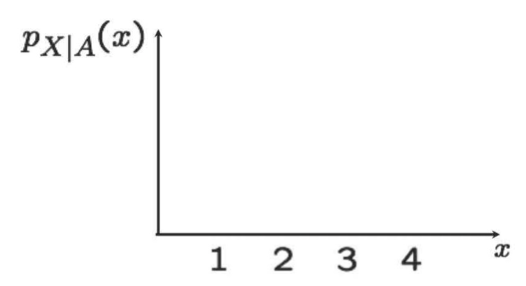
\includegraphics[width=0.55\textwidth]{L3_cond_pmf_ex2.png}
\medskip

\aleq{
\expect{X | A} = \onslide<4->{\frac{1}{3}(2+3+4) = 3}
}
\aleq{
\var{X |A} &= \onslide<5->{\expect{X^2|A}-(\expect{X|A})^2}\cr
\onslide<6->{&= \frac{1}{3}(2^2 + 3^2 + 4^2) - 3^2 = 2/3}\cr
}


}

\end{frame}

%%%%%%%%%%%%%%%%%%%%%%%%%%%%%%%%%%%%%%%%%%%%%%%%%%%%%%
\begin{frame}{Conditional PMF: Conditioning on a RV }

What do we mean by \redf{``conditioning on a rv"}? Consider $A = \{Y = y\}$ for a rv $Y.$

\medskip

\mytwocols{0.5}
{
\plitemsep 0.2in
\bci 

\item<2-> $\pxA \ \eqdef \ \cprob{X=x | A}$ 

\item<3-> $\expect{X | A} \ \eqdef \ \sum_x x \pxA$

\item<4-> $\expect{g(X) | A} \ \eqdef \ \sum_x g(x) \pxA$

\item<5-> $\var{X | A} \ \eqdef \ \expect{X^2 |A } - (\expect{X|A})^2$
\eci 
}
{
\plitemsep 0.2in
\bci 

\item<2-> $\redf{\pxcy} \ \eqdef \ \cprob{X=x |{Y = y }}$ 

\item<3-> $\redf{\expect{X | Y=y}} \ \eqdef \ \sum_x x \pxcy$

\item<4-> $\redf{\expect{g(X) | Y=y}} \ \eqdef \ \sum_x g(x) \pxcy$

\item<5-> $\redf{\var{X | Y=y}} \ \eqdef$ \\ $\expect{X^2 |Y=y } - (\expect{X|Y=y})^2$
\eci 

}

\end{frame}

%%%%%%%%%%%%%%%%%%%%%%%%%%%%%%%%%%%%%%%%%%%%%%%%%%%%%%
\begin{frame}{Conditional PMF}


\mytwocols{0.7}
{
\plitemsep 0.1in
\small

\bci 
\item \redf{Conditional PMF} 
\onslide<2->{
$$\pxcy \ \eqdef \ \cprob{X=x |{Y = y }} = \frac{\pxy}{\py}$$ 
for $y$ such that $\py >0.$}

\item<3-> $\sum_{x} \pxcy = 1$

\item \redf{Multiplication rule.}
\aleq{
\pxy &= \onslide<4->{\py \pxcy\cr    
     &= \px \pycx} 
}


\item $p_{X,Y,Z}(x,y,z) = \onslide<5->{\px \pycx p_{Z|X,Y}(z | x,y)}$
\eci 
}
{
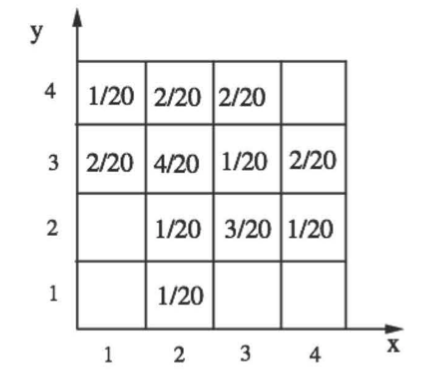
\includegraphics[width=0.5\textwidth]{L3_joint_ex.png}

\medskip
\small

$p_{X|Y}(2|2) = \frac{1}{1+3+1}$

\bigskip
$p_{X|Y}(3|2)= \frac{3}{1+3+1}$

\bigskip

$\expect{X | Y = 3} = 1(2/9)+ 2(4/9)+3(1/9)+4(2/9) $

}
\end{frame}

%%%%%%%%%%%%%%%%%%%%%%%%%%%%%%%%%%%%%%%%%%%%%%%%%%%%%%
\begin{frame}{Remind: Total Probability Theorem (from Lecture 2)}

\mytwocols{0.7}
{
\plitemsep 0.1in
\bci [$\circ$]

\item Partition of $\Omega$ into $A_1,A_2,A_3$

\item Known: $\cprob{A_i}$ and $\cprob{B | A_i}$ 

\item What is $\cprob{B}$? (probability of result)

\bigskip
\medskip

\begin{block}{Total Probability Theorem}
$$
\cprob{B} = \sum_{i} \cprob{A_i} \cprob{B | A_i}
$$
\end{block}

\eci 
}
{
\centering
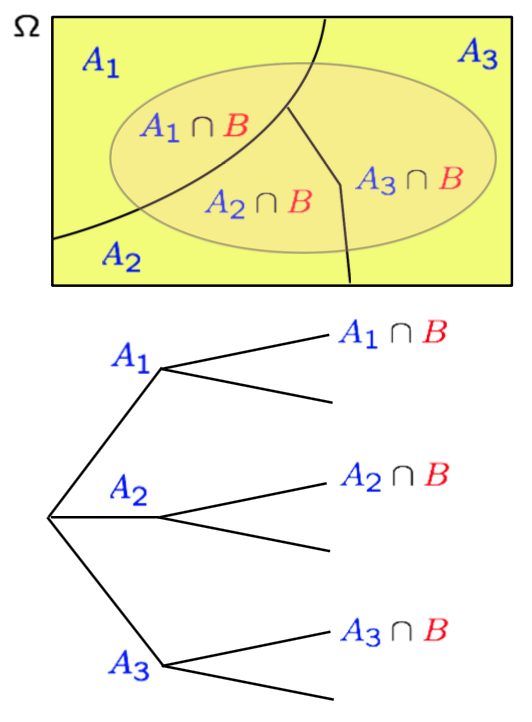
\includegraphics[width=0.65\textwidth]{L2_total_ex.png}
}

\end{frame}

%%%%%%%%%%%%%%%%%%%%%%%%%%%%%%%%%%%%%%%%%%%%%%%%%%%%%%
\begin{frame}{Total Probability Theorem: $B = \{X=x \}$}

\myvartwocols{0.7}{0.7}{0.28}
{
\plitemsep 0.1in
\bci [$\circ$]

\item Partition of $\Omega$ into $A_1,A_2,A_3$


\bigskip
\medskip

\begin{block}{Total Probability Theorem}
$$
\redf{\px} = \sum_{i} \cprob{A_i} \cprob{\redf{X=x} | A_i} = \sum_{i} \cprob{A_i} \redf{p_{X|A_i}(x)} 
$$
\end{block}

\eci 
}
{
\centering
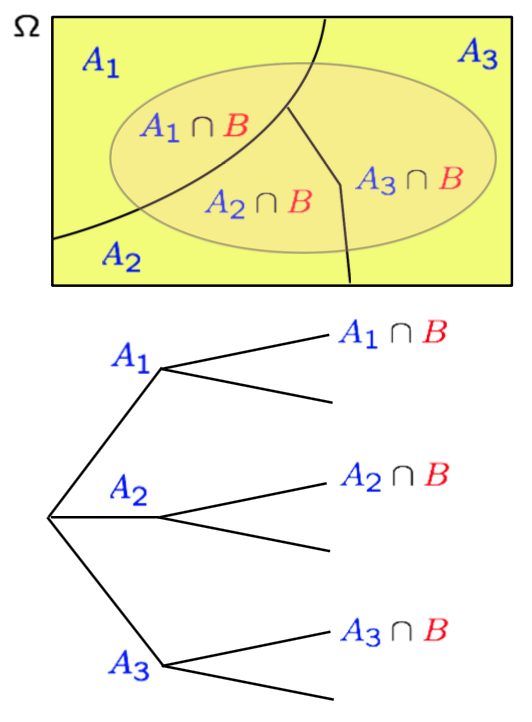
\includegraphics[width=0.8\textwidth]{L2_total_ex.png}
}

\end{frame}

%%%%%%%%%%%%%%%%%%%%%%%%%%%%%%%%%%%%%%%%%%%%%%%%%%%%%%
\begin{frame}{Total Expectation Theorem for $\{A_i \}$}

\myvartwocols{0.7}{0.7}{0.28}
{
\plitemsep 0.1in
\bci [$\circ$]

\item Partition of $\Omega$ into $A_1,A_2,A_3$


\bigskip
\medskip

\begin{block}{Total Probability Theorem}
$$
\px = \sum_{i} \cprob{A_i} \cprob{X=x | A_i} = \sum_{i} \cprob{A_i} p_{X|A_i}(x) 
$$
\end{block}

\begin{block}{Total Expectation Theorem}
$$
\expect{X} = \sum_{i} \cprob{A_i} \expect{X | A_i}
$$
\end{block}


\eci 
}
{
\centering
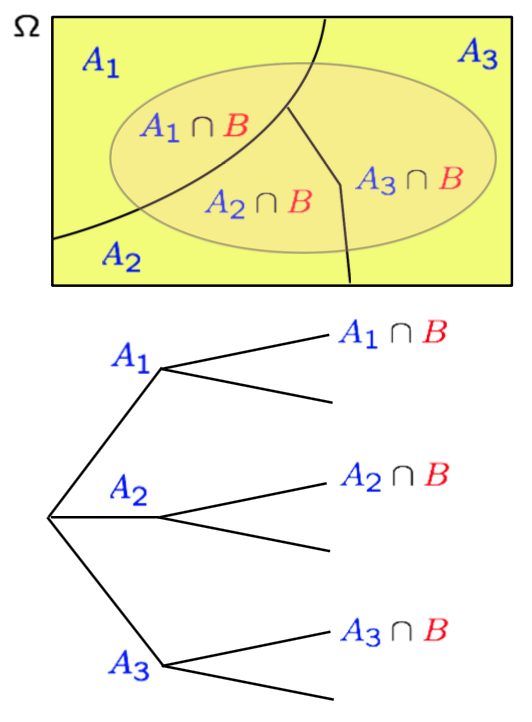
\includegraphics[width=0.8\textwidth]{L2_total_ex.png}
}

\end{frame}

%%%%%%%%%%%%%%%%%%%%%%%%%%%%%%%%%%%%%%%%%%%%%%%%%%%%%%
\begin{frame}{Total Expectation Theorem for $\{Y=y \}$}

\myvartwocols{0.7}{0.7}{0.28}
{
\plitemsep 0.1in
\bci [$\circ$]

\item Partition of $\Omega$ into $A_1,A_2,A_3$


\bigskip
\medskip

\begin{block}{Total Expectation Theorem}
$$
\expect{X} = \sum_{i} \cprob{A_i} \expect{X | A_i}
$$
\end{block}

\begin{block}<2->{Total Expectation Theorem}
$$
\expect{X} = \sum_{y} \cprob{Y=y} \expect{X | Y= y} = \sum_{y} \py \expect{X | Y=y} 
$$
\end{block}


\eci 
}
{
\centering
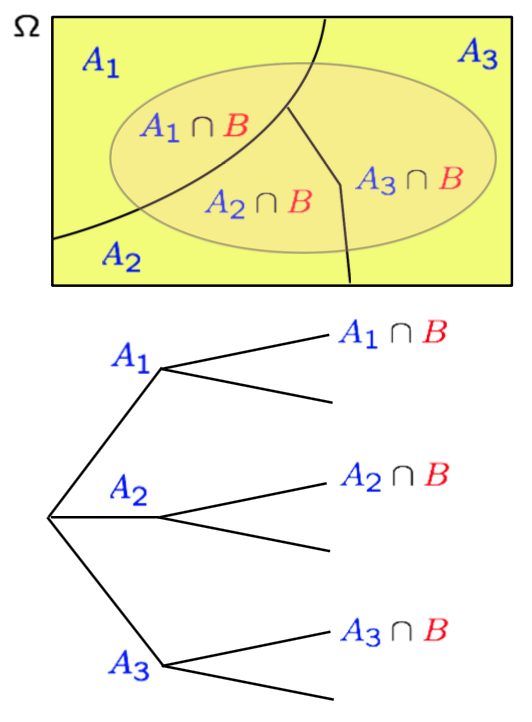
\includegraphics[width=0.8\textwidth]{L2_total_ex.png}
}

\end{frame}

%%%%%%%%%%%%%%%%%%%%%%%%%%%%%%%%%%%%%%%%%%%%%%%%%%%%%%
\begin{frame}{Example 1: Total Expectation Theorem}

\myvartwocols{0.7}{0.6}{0.38}
{
\plitemsep 0.1in
\bci 

\item $A_1 = \{X \in \{0,1,2\} \}$, $A_2 = \{ X \in \{6,7,8\} \}$ 

\item<2-> Using TET,  
\aleq{
\expect{X} &= \sum_{i=1,2}\cprob{A_i} \expect{X | A_i}\cr
&= 1/3 \cdot 1 + 2/3 \cdot 7 = 7
}
\item<3-> Without using TET, 
\aleq{
\expect{X} = \frac{1}{9}( 0 + 1 + 2) + \frac{2}{9} ( 6+7+8)
}
\eci 
}
{
\centering
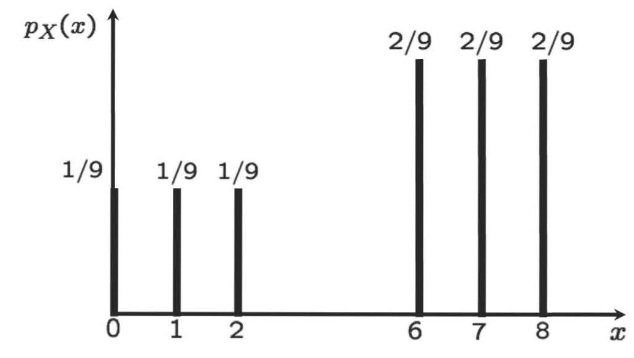
\includegraphics[width=0.95\textwidth]{L3_total_exp_ex.png}
}

\end{frame}


%%%%%%%%%%%%%%%%%%%%%%%%%%%%%%%%%%%%%%%%%%%%%%%%%%%%%%
\begin{frame}{Background: Memoryless Property of Geometric rv (1)}

\plitemsep 0.1in
\bci 

\item<1-> Some random variable often does not have \redf{memory.}

\item<2-> \bluef{Definition.} A random variable $X$ is called \redblk{memoryless} if, for any $n,m \ge 0,$ $$\cprob{X > n+m | X > m} = \cprob{X > n}$$

\item<3-> \bluef{Meaning.} Conditioned on $X > m,$ $X-m$'s distribution is the same as the original $X.$

\item<4-> \bluef{Remind.} Geometric rv $X$ with parameter $p$
\aleq{
\cprob{X = k}& = (1-p)^{k-1} p\cr
\cprob{X > k}& = 1 - \sum_{k'=1}^k (1-p)^{k'-1} p = (1-p)^k
}
\eci

\end{frame}

%%%%%%%%%%%%%%%%%%%%%%%%%%%%%%%%%%%%%%%%%%%%%%%%%%%%%%
\begin{frame}{Background: Memoryless Property of Geometric rv (2)}

\plitemsep 0.3in
\bci 

\item \bluef{Theorem.} Any geometric random variable is \redf{memoryless.}

\onslide<2->{
\begin{align*}
\cprob{X > n+m | X > m} &= \frac{\cprob{X > n+m \text{ and } X > m}}{\cprob{X > m}} \cr
& = \frac{\cprob{X > n+m}}{\cprob{X > m}}\cr
& = \frac{(1-p)^{n+m}}{(1-p)^m} = (1-p)^n = \cprob{X >n}
\end{align*}}

\item<3-> \bluef{Meaning.} Conditioned on $X > m,$ $X-m$ is geometric with the same parameter. 


\eci

\end{frame}


%%%%%%%%%%%%%%%%%%%%%%%%%%%%%%%%%%%%%%%%%%%%%%%%%%%%%%
\begin{frame}{Example 2: Mean and Variance of Geometric rv}

\mytwocols{0.8}
{
\plitemsep 0.1in
\small
\bci 

\item<1-> Write softwares over and over, and each time w.p. $p$ of working correctly (independent from prev. programs). 

\item<2-> $X$: number of tries until the program works correctly. 

\item<3-> \redf{Q) mean and variance of $X$}

\item<4-> $X$ is geometric

\item<5-> Direct computation is boring.
\aleq{
\expect{X} = \sum_{k=1}^\infty k(1-p)^{k-1} p
}

\item<6-> Total expectation theorem and memorylessness nhelps a lot. 
\eci
}
{
\plitemsep 0.1in

\bci 

\item<7-> $A_1 = \{X=1 \}$ (first try is success), $A_2 = \{X >1 \}$ (first try is failure).  

\begin{align*}
    \expect{X} & = 1 + \expect{X-1} \cr
 &= \onslide<8->{1 + \cprob{A_1} \expect{X-1 | X=1} \cr
 &\text{              }+ \cprob{A_2} \expect{X-1 | X >1}}\cr
&= \onslide<9->{1 + (1-p) \expect{X}}
\end{align*}

\onslide<10->{$\expect{X} = 1+(1-p)\frac{1}{p} = 1/p.$}
\eci
}

\end{frame}

%%%%%%%%%%%%%%%%%%%%%%%%%%%%%%%%%%%%%%%%%%%%%%%%%%%%%%
\begin{frame}{Roadmap}

\plitemsep 0.1in

\bci [$\circ$]
\item \bluef{Famous discrete random variables used in the community

- Bernoulli, Uniform, Binomial, Geometric, Poisson, etc. }

\item \bluef{Summarizing a random variable: Expectation and Variance}

\item \bluef{Functions of a single random variable}, \bluef{Functions of multiple random variables} 

\item \bluef{Conditioning for random variables}, \redf{Independence for random variables} 

\item Continuous random variables

- Normal, Uniform, Exponential, etc. 

\item Bayes' rule for random variables
\eci 

\end{frame}

%%%%%%%%%%%%%%%%%%%%%%%%%%%%%%%%%%%%%%%%%%%%%%%%%%%%%%
\begin{frame}{Independence, Conditional Independence}

\plitemsep -0.1in

\bci 
\item<2-> Two events
\aleq{
\cprob{A \cap B} &= \cprob{A} \cdot \cprob{B} \cr
\cprob{A \cap B \redf{| C}} &= \cprob{A \redf{|C}} \cdot \cprob{B \redf{|C}}
}

\item<3-> A rv and an event
\aleq{
\cprob{ \{X = x \} \cap B} &= \cprob{X=x} \cdot \cprob{B}, \quad \text{for all $x$} \cr
\cprob{ \{X = x \} \cap B\redf{| C} } &= \cprob{X=x\redf{| C}} \cdot \cprob{B\redf{| C}}, \quad \text{for all $x$}
}

\item<4-> Two rvs
\aleq{
\cprob{ \{X = x \} \cap \{Y=y \}} &= \cprob{X=x} \cdot \cprob{Y=y}, \quad \text{for all $x,y$}\cr
\onslide<5->{\pxy&= \px \cdot \py}
}
\aleq{
\cprob{ \{X = x \} \cap \{Y=y \}\redf{|{Z=z}}} &= \cprob{X=x\redf{|{Z=z}}} \cdot \cprob{Y=y\redf{|{Z=z}}}, \quad \text{for all $x,y$}\cr
\onslide<5->{p_{X,Y\redf{|Z}}(x,y)&=p_{X\redf{|Z}}(x) \cdot p_{Y\redf{|Z}}(y)}
}

\eci 

\end{frame}

%%%%%%%%%%%%%%%%%%%%%%%%%%%%%%%%%%%%%%%%%%%%%%%%%%%%%%
\begin{frame}{Example}


\mytwocols{0.7}
{
\plitemsep 0.4in
\bci 

\item $X \indep Y$?
\onslide<2->{
\aleq{
p_{X,Y}(1,1) = 0,& \quad p_X(1) = 3/20\cr
p_Y{1} = 1/20.&
}}

\item $X \indep Y | \{X \leq 2\text{ and } Y \ge 3\}$?

\onslide<3->{- Yes.}

\eci 
}
{
\centering
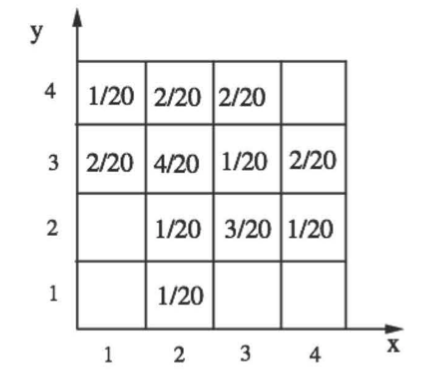
\includegraphics[width=0.6\textwidth]{L3_joint_ex.png}

\medskip

\small
\onslide<3->{
\begin{tabular}{|c|c|c|} \hline 
$Y=4$ (1/3)& 1/9 & 2/9\\ \hline
$Y=3$ (2/3)& 2/9& 4/9\\ \hline
& $X=1$ (1/3)&$X=2 (2/3)$ \\ \hline
\end{tabular}
}
}
\end{frame}

%%%%%%%%%%%%%%%%%%%%%%%%%%%%%%%%%%%%%%%%%%%%%%%%%%%%%%
\begin{frame}{Expectation and Variance}

\mytwocols{0.8}
{
%\small
\plitemsep 0.05in
\bci 

\item<1-> Always true. 

$\expect{aX +b}$, $\expect{X+Y} = \expect{X} + \expect{Y}$

\item<2-> Generally,
$\expect{g(X,Y)} \neq g(\expect{X},\expect{Y})$

\medskip

\item<3-> However, if $X \indep Y,$
\aleq{
\expect{XY} &= \expect{X} \expect{Y} \cr
\expect{g(X)h(Y)} &= \expect{g(X)} \expect{g(Y)}
}
\item<4-> \bluef{Proof.}
\aleq{
\expect{g(X)h(Y)} &= \sum_{x}\sum_{y} g(x)h(y) \pxy \cr
&= \sum_x x \px \sum_y y \py
}

\eci
}
{
\plitemsep 0.1in
\bci 

\item<5-> Always true. 

$\var{aX} = a^2 \var{X}$, $\var{X + a} = \var{X}$

\item<6-> Generally,
$\var{X+Y} \neq \var{X} + \var{Y}$

\medskip

\item<7-> However, if $X \indep Y,$
\aleq{
\var{X+Y} &= \var{X} + \var{Y}
}

\item<7-> Practice.

\plitemsep 0.02in
\bci
\item<8-> $X=Y$ $\imp$ $\var{X+Y} = 4 \var{X}$
\item<9-> $X=-Y$ $\imp$ $\var{X+Y} = 0$
\item<10-> $X \indep Y$ $\imp$ $\var{X-3Y} = \var{X} + 9 \var{Y}$
\eci

\eci

}
\end{frame}


%%%%%%%%%%%%%%%%%%%%%%%%%%%%%%%%%%%%%%%%%%%%%%%%%%%%%%
\begin{frame}{$\var{X + Y} \neq \var{X} + \var{Y}$}

\plitemsep 0.1in
\bci [$\circ$]

\item<1-> Why not generally true?

\onslide<2->{
\aleq{
\var{X+Y} &= \expect{(X+Y)^2} - (\expect{X+Y})^2 \cr
& = \expect{X^2 + Y^2 + 2XY} - \left( (\expect{X})^2 +(\expect{Y})^2 + 2 \expect{X}\expect{Y} \right ) \cr
& = \var{X} + \var{Y} +2 \left(\expect{XY} - \expect{X}\expect{Y} \right)
}}

\item<3-> \redblank{4}{$X \indep Y$} is a sufficient condition for $\expect{XY} = \expect{X}\expect{Y}$ 

\item<5-> Also, a necessary condition? we will see later, when we study \redf{covariance.} 
\eci

\end{frame}

%%%%%%%%%%%%%%%%%%%%%%%%%%%%%%%%%%%%%%%%%%%%%%%%%%%%%%
\begin{frame}{Example: The hat problem (1)}

\plitemsep 0.1in
\bci 
\item<1-> $n$ people throw their hats in a box and then pick one at random

\item<1-> $X$: number of people with their own hat

\item<2->  $\redf{\expect{X}}$? $\redf{\var{X}}$?

\item<3-> All permutations are equally likely as $1/n!.$ Thus, this equals to picking one hat at a time.

\item<4-> \bluef{Key step 1.} Define a rv $X_i=1$ if $i$ selects own hat and $0$ otherwise. 
$$X = \sum_{i=1}^n X_i.$$

\item<5-> $\{X_i\}, i=1, 2, \ldots, n$: identically distributed (symmetry)

% \item $\expect{X} = n \expect{X_1} = n \cprob{X_1 =1} = 1/n.$

% \item \bluef{Key step 2.} Are $X_i$s are independent? If yes, easy to get $\cvar{X}.$

\eci
\end{frame}

%%%%%%%%%%%%%%%%%%%%%%%%%%%%%%%%%%%%%%%%%%%%%%%%%%%%%%
\begin{frame}{Example: The hat problem (2)}

\plitemsep 0.05in
\bci 
\item<1-> $\expect{X} = n \expect{X_1} = n \cprob{X_1 =1} = n\times \frac{1}{n} = 1.$

\item<2-> \bluef{Key step 2.} Are $X_i$s are independent? If yes, easy to get $\cvar{X}.$

\item<3-> Assume $n=2.$ Then, $X_1=1 \rightarrow X_2=1,$ and $X_1=0 \rightarrow X_2=0.$ Thus, \redf{dependent}.
\aleq{
\onslide<4->{\cvar{X} &= \expect{X^2} - (\expect{X})^2 \cr
&= \bexpect{\sum_{i}X_i^2 + \sum_{i,j:i\neq j} X_i X_j} - (\expect{X})^2}\cr
\onslide<5->{\expect{X_i^2} &= 1 \times \frac{1}{n} + 0 \times \frac{n-1}{n} = \frac{1}{n}}\cr
\onslide<6->{\expect{X_i X_j} &= \expect{X_1 X_2} = 1 \times \cprob{X_1 X_2 = 1} = \cprob{X_1=1}\cprob{X_2 =1 | X_1 =1}, \quad \text{($i \neq j$)}}
}

\item<7-> $\expect{X^2} = n \expect{X_1^2} + n(n-1) \expect{X_1 X_2} = n\frac{1}{n} + n(n-1)\frac{1}{n(n-1)} = 2$

\item<8-> $\cvar{X} = 2-1 =1$
\eci
\end{frame}


%%%%%%%%%%%%%%%%%%%%%%%%%%%%%%%%%%%%%%%%%%%%%%%%%%%%%%
\begin{frame}{}
\vspace{2cm}
\LARGE Questions?

\end{frame}

\begin{frame}{Review Questions}

\bce[1)]
\item What is Random Variable? Why is it useful?

\item What is PMF (Probability Mass Function)?

\item Explain Bernoulli, Binomial, Poisson, Geometric rvs, when they are used and what their PMFs are. 

\item What are joint and marginal PMFS?

\item Describe and explain the total probability/expectation theorem for random variables?

\item When is it useful to use total probability/expectation theorem?

\item What is conditional independence? 
\ece
\end{frame}



\end{document}
